% Positioning of Parts II--IV: layer (rows) x what is sharded (columns)
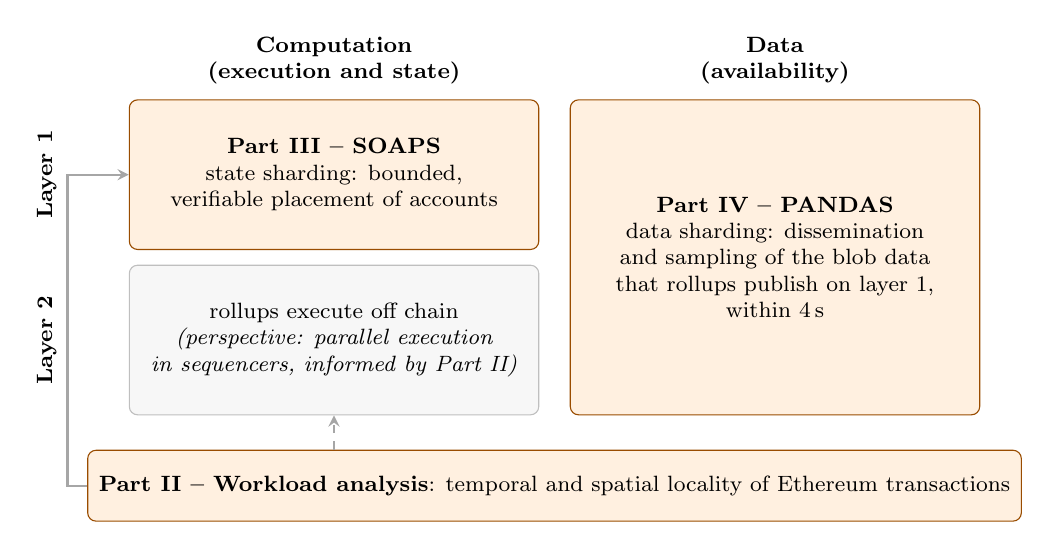
\begin{tikzpicture}[x=1cm,y=1cm,font=\footnotesize,
	cell/.style={draw=gray!50,rounded corners=3pt,minimum width=5.2cm,minimum height=1.9cm,align=center,inner sep=4pt},
	head/.style={font=\footnotesize\bfseries,align=center},
	contrib/.style={fill=orange!12,draw=orange!60!black},
	other/.style={fill=gray!6},
	link/.style={->,>=stealth,thick,gray!70,dashed}]

	% column and row headers
	\node[head] at (0,2.4) {Computation\\(execution and state)};
	\node[head] at (5.6,2.4) {Data\\(availability)};
	\node[head,rotate=90] at (-3.65,0.95) {Layer 1};
	\node[head,rotate=90] at (-3.65,-1.15) {Layer 2};

	% layer 1
	\node[cell,contrib] (soaps) at (0,0.95)
		{\textbf{Part III -- SOAPS}\\state sharding: bounded,\\verifiable placement of accounts};
	\node[cell,contrib,minimum height=4.0cm] (pandas) at (5.6,-0.1)
		{\textbf{Part IV -- PANDAS}\\data sharding: dissemination\\and sampling of the blob data\\that rollups publish on layer~1,\\within 4\,s};

	% layer 2
	\node[cell,other] (rollups) at (0,-1.15)
		{rollups execute off chain\\{\itshape (perspective: parallel execution}\\{\itshape in sequencers, informed by Part II)}};

	% Part II informs computation
	\node[cell,contrib,minimum width=10.8cm,minimum height=0.9cm] (workload) at (2.8,-3.0)
		{\textbf{Part II -- Workload analysis}: temporal and spatial locality of Ethereum transactions};
	% Part II informs state placement (main use) and parallel execution (perspective)
	\draw[link,solid] (workload.west) -- ++(-0.25,0) |- (soaps.west);
	\draw[link] (workload.north -| rollups.south) -- (rollups.south);
\end{tikzpicture}
